% NI-SORF prediction speedup note (standalone Overleaf document).
% Compile with pdfLaTeX (TikZ requires no extra install on Overleaf).
\documentclass[11pt]{article}

\usepackage[margin=1in]{geometry}
\usepackage{amsmath,amssymb,mathtools}
\usepackage{booktabs}
\usepackage{tabularx}
\usepackage{graphicx}
\usepackage{hyperref}
\usepackage{xcolor}
\usepackage{caption}
\usepackage{enumitem}
\usepackage{placeins}
\usepackage{tikz}
\usepackage{pgfplots}
\pgfplotsset{compat=1.17}
\usetikzlibrary{arrows.meta,positioning,calc,chains}

\hypersetup{colorlinks=true, linkcolor=blue!55!black, urlcolor=blue!55!black}

\newcommand{\gradmu}{\nabla_{x}\mu}
\newcommand{\homo}{w_{\mathrm{homo}}}
\newcommand{\Phitr}{\Phi}
\newcommand{\phistar}{\varphi}

\title{Why NI-SORF Prediction Got Much Faster\\[0.35em]
\large Same NIGP math, far less repeated linear algebra}
\author{Tyler Johnson\\
\small SpectralGPPlus / EMIT S4 independent SORF+NIGP}
\date{}

\begin{document}
\maketitle

\begin{abstract}
\noindent
NIGP-enabled SORF prediction on the S4 EMIT suite (\textbf{7} independent QoI models,
$\sim$10k train / 25k test) was slow for two engineering reasons---not because of the
Mat\'ern-3/2 kernel. We (1)~amortize the expensive train-side Woodbury solve used for
$\gradmu$ so it runs \emph{once per QoI} instead of once per test chunk, and
(2)~optionally parallelize prediction across QoIs while reporting wall-clock time.
NIGP formulas for the mean and observation intervals are unchanged.
\end{abstract}

\section{Bottom line}

Prediction was slow for two separate reasons. We fixed both.
\textbf{NIGP math did not change}---we still use train-side effective noise for the
predictive mean and test-side $\gradmu$ for observation uncertainty.

\begin{center}
\small
\begin{tabularx}{\textwidth}{@{}>{\raggedright\arraybackslash}p{0.32\textwidth}
  >{\raggedright\arraybackslash}p{0.32\textwidth}
  >{\raggedright\arraybackslash}X@{}}
\toprule
\textbf{What was wrong} & \textbf{What we did} & \textbf{Effect} \\
\midrule
Same train-side Woodbury solve for $\homo$ repeated $\sim$13$\times$ per QoI while
walking over test chunks
& Solve $\homo$ \textbf{once}, reuse for every test batch
& Largest single-model win ($\sim$4$\times$ at matched $D{=}2400$:
$\sim$18.5\,s $\to$ $\sim$4.66\,s per QoI; full 7 QoIs
$\sim$127\,s $\to$ $\sim$33\,s wall) \\[0.6em]
Seven QoIs predicted sequentially; cost table \emph{summed} those timers
& Optional \textbf{parallel} predict across QoIs; report \textbf{wall-clock} for all~7
& Cuts total wait on CPU / multi-GPU; fairer ``all QoIs ready'' metric \\
\bottomrule
\end{tabularx}
\end{center}

\vspace{0.5em}
\paragraph{Not Mat\'ern-3/2.}
\texttt{spectral\_kernel=matern32} only changes how random frequencies are sampled at
initialization. After that, featurize / Woodbury / $\gradmu$ match RBF.
Older cost slides also compared Mat3/2 at \textbf{$D{=}2400$} to RBF at
\textbf{$D{=}2000$}, which alone looks $\sim$40\% slower because Gram/Cholesky cost
scales roughly like $D^2$.

\section{What NIGP needs at predict time}

NIGP turns input noise into extra observation noise using the slope of the
predictive mean. With input-noise covariance $\Sigma_x$,
\begin{equation}
\label{eq:d-eff}
  d(x)
  \;=\;
  \sigma_y^2
  +
  \bigl(\gradmu(x)\bigr)^{\!\top}
  \Sigma_x\,
  \gradmu(x).
\end{equation}
Train-side $d$ enters the predictive \textbf{mean}; test-side $d$ enters
\textbf{observation} intervals (NIS / coverage).

\subsection Homoskedastic feature weights $\homo$

For RFF/SORF, write scaled train features as $\Phitr\in\mathbb{R}^{n\times m}$
($m=2D$) and centered targets $y_c=y-m(X)$. The slope $\gradmu$ is
\emph{not} differentiated through the NIGP $d$; it uses a frozen dual weight
vector from the \textbf{homoskedastic} model $\Sigma=\sigma_y^2 I_n+\Phitr\Phitr^{\top}$:
\begin{equation}
\label{eq:Lambda-homo}
  \Lambda
  \;=\;
  \Phitr^{\top}\Phitr + \sigma_y^2 I_m,
\end{equation}
\begin{equation}
\label{eq:w-homo}
  \homo
  \;=\;
  \Lambda^{-1}\Phitr^{\top} y_c.
\end{equation}
(Equivalently $\homo$ solves the dual Woodbury system; we Cholesky-factor $\Lambda$ once.)
The posterior mean at a point $x$ is then
\begin{equation}
\label{eq:mu-rff}
  \mu(x)
  \;=\;
  m(x) + \phistar(x)^{\top}\homo,
\end{equation}
where $\phistar(x)\in\mathbb{R}^{m}$ are the scaled RFF features of $x$. Differentiating
only through $m$ and $\phistar$ (with $\homo$ held fixed) gives the analytic Jacobian
$\gradmu(x)$ used in~\eqref{eq:d-eff}.

\paragraph{Why this was expensive.}
Forming/factoring $\Lambda$ is $O(n m^2+m^3)$. That is the ``heavy solve'' we
must not repeat unnecessarily. (This $\homo$ is \emph{not} the RFF frequency matrix
$\Omega$; frequencies only appear inside $\phistar$.)

\section{The old bottleneck (and the fix)}

With chunked test evaluation (e.g.\ chunk size 2048 $\Rightarrow$
$\lceil 25000/2048\rceil=13$ chunks), the old path re-featurized the \emph{full}
training set and \textbf{re-solved}~\eqref{eq:w-homo} on every chunk. Logging and
plotting were never inside \texttt{Prediction\_Time}.

\begin{figure}[t]
\centering
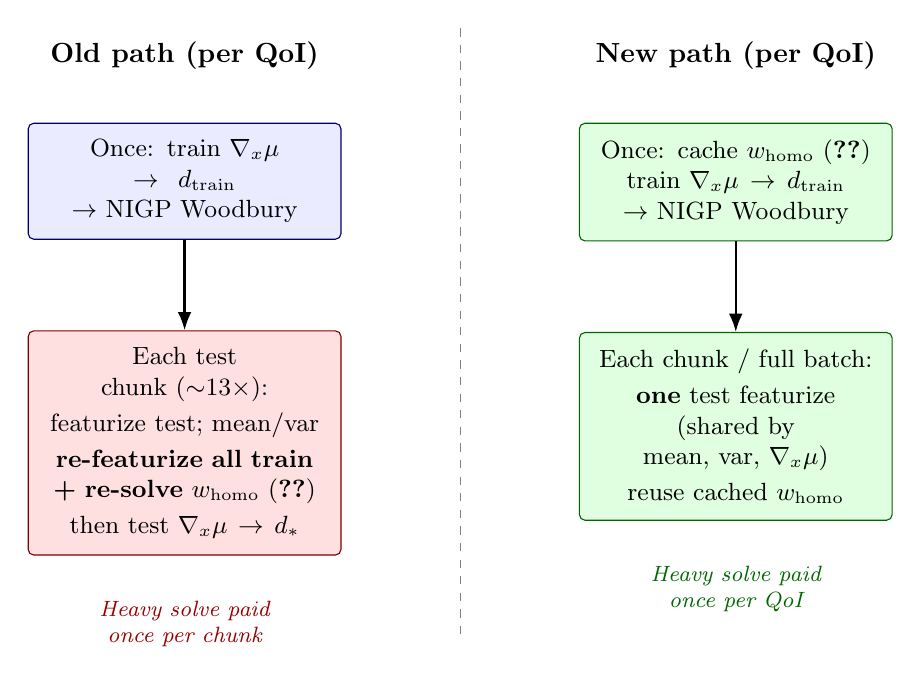
\begin{tikzpicture}[
  font=\small,
  node distance=1.15cm,
  box/.style={draw, rounded corners=2pt, align=center, inner sep=6pt,
              text width=3.55cm, minimum height=1.15cm},
  waste/.style={box, fill=red!12, draw=red!50!black},
  good/.style={box, fill=green!12, draw=green!40!black},
  once/.style={box, fill=blue!8, draw=blue!40!black},
  arr/.style={-{Latex}, thick},
  note/.style={font=\itshape\footnotesize, align=center, text width=3.55cm},
]
% --- OLD column ---
\node[font=\bfseries] (oldtitle) at (0,0) {Old path (per QoI)};
\node[once, below=0.55cm of oldtitle] (o1)
  {Once: train $\gradmu$\\$\to d_{\mathrm{train}}$\\$\to$ NIGP Woodbury};
\node[waste, below=of o1] (o2)
  {Each test chunk ($\sim$13$\times$):\\[2pt]
   featurize test; mean/var\\[2pt]
   \textbf{re-featurize all train}\\
   \textbf{+ re-solve $\homo$~\eqref{eq:w-homo}}\\[2pt]
   then test $\gradmu\to d_*$};
\draw[arr] (o1) -- (o2);
\node[note, text=red!60!black, below=0.45cm of o2] (onote)
  {Heavy solve paid once per chunk};

% --- NEW column ---
\node[font=\bfseries] (newtitle) at (7.0,0) {New path (per QoI)};
\node[good, below=0.55cm of newtitle] (n1)
  {Once: cache $\homo$~\eqref{eq:w-homo}\\
   train $\gradmu\to d_{\mathrm{train}}$\\
   $\to$ NIGP Woodbury};
\node[good, below=of n1] (n2)
  {Each chunk / full batch:\\[2pt]
   \textbf{one} test featurize\\
   (shared by mean, var, $\gradmu$)\\[2pt]
   reuse cached $\homo$};
\draw[arr] (n1) -- (n2);
\node[note, text=green!40!black, below=0.45cm of n2] (nnote)
  {Heavy solve paid once per QoI};

\draw[dashed, gray] ($(oldtitle)!0.5!(newtitle) + (0,0.35)$)
  -- ($(onote)!0.5!(nnote) + (0,-0.35)$);
\end{tikzpicture}
\caption{Amortizing NIGP predict: remove redundant evaluations of~\eqref{eq:w-homo}
inside the test loop. Default S4 also uses a single full-test batch
(\texttt{PREDICT\_CHUNK\_SIZE\,=\,0}) when GPU memory allows.}
\label{fig:amortize}
\end{figure}

\FloatBarrier

\section{Correctness (what stayed the same)}

\begin{itemize}[leftmargin=1.2em,itemsep=0.25em]
  \item Train NIGP $d$ from~\eqref{eq:d-eff} still builds the predictive mean
        (diag-noise Woodbury with $d_{\mathrm{train}}$).
  \item Test NIGP $d_*$ still builds observation intervals.
  \item Cached vs recomputed $\homo$, and chunked vs full-batch predict, match to
        tight numerical tolerance in unit tests.
\end{itemize}

\section{Parallel prediction across QoIs}

Each QoI is its own \texttt{RFFGPR}. Training remains sequential. After training we
stash models on CPU and run a dedicated \textbf{predict phase}.

\begin{figure}[t]
\centering
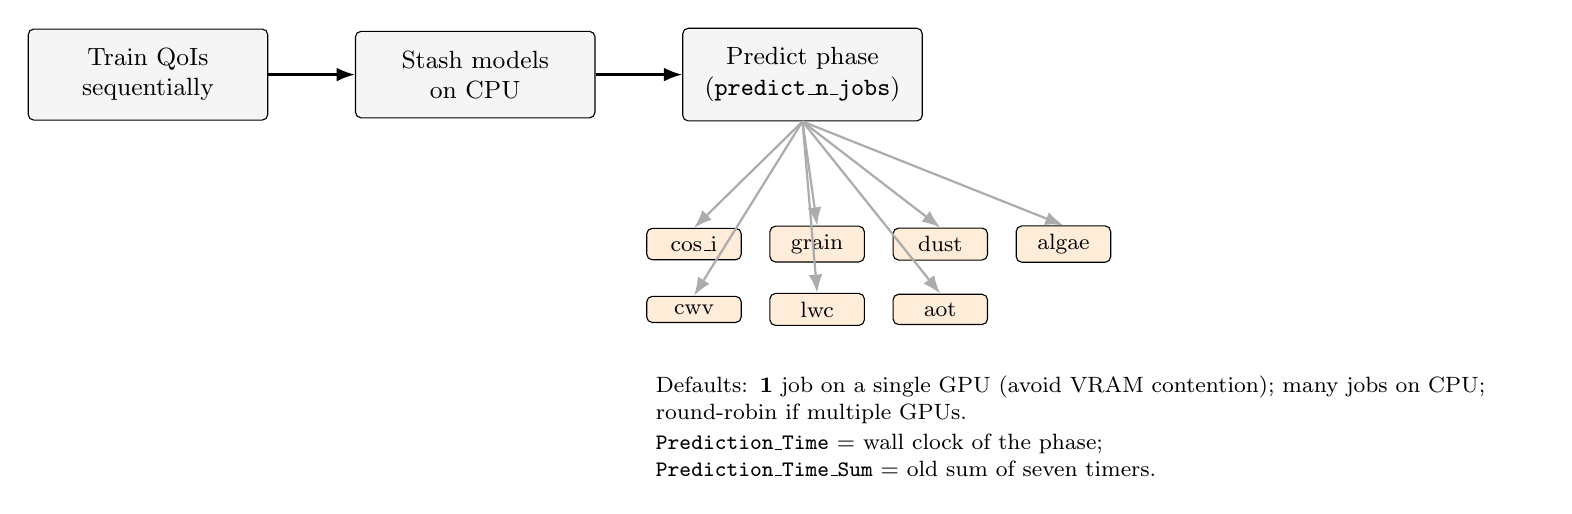
\begin{tikzpicture}[
  font=\small,
  node distance=1.35cm and 1.1cm,
  stage/.style={draw, rounded corners=2pt, align=center, inner sep=7pt,
                fill=gray!8, text width=2.55cm, minimum height=1.0cm},
  qoi/.style={draw, rounded corners=2pt, align=center, inner sep=3pt,
              fill=orange!15, minimum width=1.2cm, font=\footnotesize},
  arr/.style={-{Latex}, thick},
]
\node[stage] (train) {Train QoIs\\sequentially};
\node[stage, right=of train] (stash) {Stash models\\on CPU};
\node[stage, right=of stash] (pred) {Predict phase\\(\texttt{predict\_n\_jobs})};

\draw[arr] (train) -- (stash);
\draw[arr] (stash) -- (pred);

\begin{scope}[node distance=0.35cm]
  \node[qoi, below=1.35cm of pred.south west, xshift=0.15cm] (q0) {cos\_i};
  \node[qoi, right=of q0] (q1) {grain};
  \node[qoi, right=of q1] (q2) {dust};
  \node[qoi, right=of q2] (q3) {algae};
  \node[qoi, below=0.45cm of q0] (q4) {cwv};
  \node[qoi, right=of q4] (q5) {lwc};
  \node[qoi, right=of q5] (q6) {aot};
\end{scope}
\foreach \q in {q0,q1,q2,q3,q4,q5,q6} {
  \draw[arr, gray!65] (pred.south) -- (\q.north);
}

\node[font=\footnotesize, align=left, text width=0.92\textwidth,
      below=0.55cm of q4.south west, anchor=north west] {
  Defaults: \textbf{1} job on a single GPU (avoid VRAM contention);
  many jobs on CPU; round-robin if multiple GPUs.\\[0.2em]
  \texttt{Prediction\_Time} $=$ wall clock of the phase;\\
  \texttt{Prediction\_Time\_Sum} $=$ old sum of seven timers.
};
\end{tikzpicture}
\caption{Two-phase emit: train all QoIs, then fan out prediction. On one busy GPU,
parallel jobs rarely beat sequential wall time; the metric still matches
deploy-style ``all QoIs ready,'' and CPU/multi-GPU benefit.}
\label{fig:parallel}
\end{figure}

\FloatBarrier

\section{Numbers (order of magnitude)}

Same problem class: NIGP on, 25k test points, 7 QoIs
(\texttt{cos\_i}, \texttt{grain\_size}, \texttt{dust}, \texttt{algae}, \texttt{cwv},
\texttt{lwc}, \texttt{aot}) unless noted. Sept18 headline run uses RBF SORF,
$D{=}2400$, amortized full-batch predict, \texttt{predict\_n\_jobs}${}={}$1 on GPU.

\begin{table}[ht]
\centering
\small
\caption{Predict times before/after amortization (matched $D{=}2400$ highlighted).}
\label{tab:times}
\begin{tabular}{@{}llrrr@{}}
\toprule
Run & Notes & $D$ & Per QoI & All 7 \\
\midrule
Sept09 Mat3/2 (old) & chunked, re-solve each chunk & 2400 & $\sim$18.5\,s & $\sim$127\,s (sum) \\
\textbf{Sept18 RBF (new)} & \textbf{amortized, full 7 QoIs} & \textbf{2400} &
  \textbf{$\sim$4.66\,s} & \textbf{$\sim$33\,s wall} \\
Sept18 Mat3/2 (new) & amortized, 1 QoI only & 2400 & $\sim$4.7\,s & --- \\
Sept09 Mat3/2 (old) & matched $D$ vs RBF & 2000 & $\sim$13\,s & $\sim$91\,s (sum) \\
Sept08 NI-SORF RBF (old) & & 2000 & $\sim$13\,s & $\sim$89\,s (sum) \\
Sept08 SORF, no NIGP & no $\gradmu$ path & 2000 & $\sim$4\,s & $\sim$28\,s (sum) \\
Sept13 speedup test & GPU, jobs$=$1, full-batch & 1000 & $\sim$0.96\,s & $\sim$7\,s wall \\
\bottomrule
\end{tabular}
\end{table}

\begin{table}[ht]
\centering
\small
\caption{Sept18 amortized run ($D{=}2400$, RBF, 7 QoIs): per-QoI
\texttt{Prediction\_Time} and suite totals.}
\label{tab:sept18-7qoi}
\begin{tabular}{@{}lr@{}}
\toprule
QoI / aggregate & Predict (s) \\
\midrule
\texttt{cos\_i} & 4.68 \\
\texttt{grain\_size} & 4.63 \\
\texttt{dust} & 4.63 \\
\texttt{algae} & 4.63 \\
\texttt{cwv} & 4.69 \\
\texttt{lwc} & 4.69 \\
\texttt{aot} & 4.69 \\
\midrule
Mean per QoI & 4.66 \\
\texttt{Prediction\_Time\_Sum} & 32.65 \\
\texttt{Prediction\_Time} (wall) & 32.96 \\
\bottomrule
\end{tabular}
\end{table}

\begin{figure}[ht]
\centering
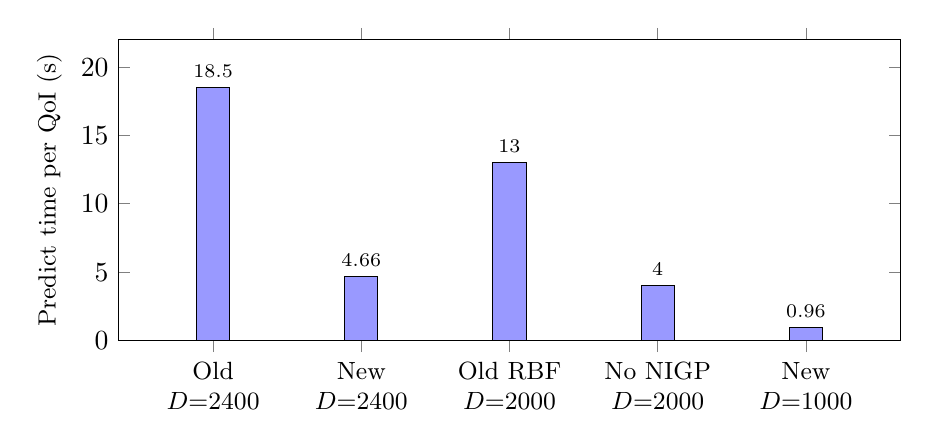
\begin{tikzpicture}
\begin{axis}[
  ybar,
  bar width=12pt,
  width=0.95\textwidth,
  height=5.4cm,
  ylabel={Predict time per QoI (s)},
  symbolic x coords={Old2400,New2400,Old2000,NoNIGP,Sept13},
  xtick=data,
  x tick label style={font=\small, align=center},
  xticklabels={Old\\$D{=}2400$, New\\$D{=}2400$, Old RBF\\$D{=}2000$,
               No NIGP\\$D{=}2000$, New\\$D{=}1000$},
  ymin=0, ymax=22,
  enlarge x limits=0.16,
  nodes near coords,
  every node near coord/.append style={font=\scriptsize},
  ylabel style={font=\small},
]
\addplot[fill=blue!40] coordinates {
  (Old2400,18.5) (New2400,4.66) (Old2000,13) (NoNIGP,4) (Sept13,0.96)
};
\end{axis}
\end{tikzpicture}
\caption{Matched-$D$ story at 2400 RFF: amortized path cuts per-QoI predict from
$\sim$18.5\,s to $\sim$4.66\,s (Sept18, mean over 7 QoIs). Smaller $D$ and
full-batch evaluation push further toward $\sim$1\,s/QoI.}
\label{fig:bars}
\end{figure}

\begin{figure}[ht]
\centering
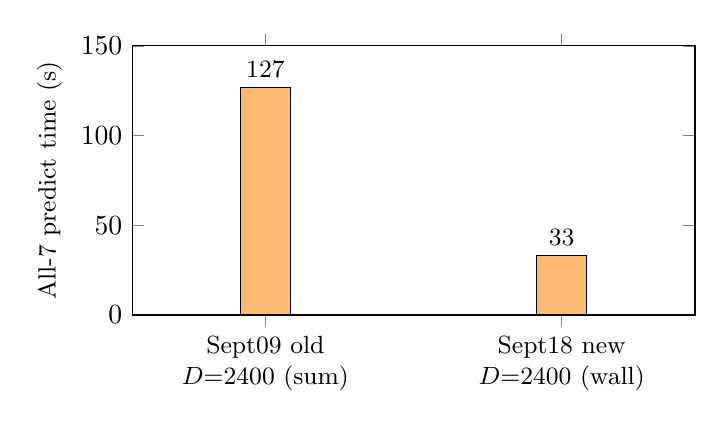
\begin{tikzpicture}
\begin{axis}[
  ybar,
  bar width=18pt,
  width=0.72\textwidth,
  height=5.0cm,
  ylabel={All-7 predict time (s)},
  symbolic x coords={Old2400,New2400},
  xtick=data,
  x tick label style={font=\small, align=center},
  xticklabels={Sept09 old\\$D{=}2400$ (sum), Sept18 new\\$D{=}2400$ (wall)},
  ymin=0, ymax=150,
  enlarge x limits=0.45,
  nodes near coords,
  every node near coord/.append style={font=\small},
  ylabel style={font=\small},
]
\addplot[fill=orange!55] coordinates {
  (Old2400,127) (New2400,33)
};
\end{axis}
\end{tikzpicture}
\caption{Full 7-QoI suite at matched $D{=}2400$: $\sim$127\,s (old sum) $\to$
$\sim$33\,s (Sept18 wall), about \textbf{3.9$\times$} faster for ``all QoIs ready.''}
\label{fig:bars-suite}
\end{figure}

\paragraph{Takeaway.}
Removing redundant evaluations of~\eqref{eq:w-homo} brings NIGP predict near the
``SORF without NIGP'' regime for a given $D$. At matched $D{=}2400$ the gain is
about \textbf{4$\times$} per QoI and \textbf{$\sim$3.9$\times$} for the full
7-QoI suite ($\sim$127\,s $\to$ $\sim$33\,s).

\section{One-sentence version (for a talk)}

\begin{quote}
We stopped re-solving $\homo=\Lambda^{-1}\Phitr^{\top}y_c$ on every test chunk,
reused one featurize for mean and NIGP slopes, optionally predict all QoIs
together, and report wall-clock---so NIGP inference is the same math with far
less repeated linear algebra.
\end{quote}

\section*{Code pointers}
\begin{itemize}[leftmargin=1.2em,itemsep=0.2em]
  \item Amortized NIGP predict:
        \texttt{gpplus/utils/nigp\_utils.py} (\texttt{feature\_weights}),
        \texttt{gpplus/training/eval.py},
        \texttt{gpplus/models/rff\_gpr.py}
  \item Two-phase + parallel QoIs:
        \texttt{experiments\_SORF/emit\_s4\_sorf\_base.py},
        \texttt{S4\_emit\_SORF.py} (\texttt{PREDICT\_CHUNK\_SIZE}, \texttt{PREDICT\_N\_JOBS})
  \item Cost-slide label:
        \texttt{render\_icy\_rrmse\_nis\_tables.py}
        (\texttt{wall 7-QoI (parallel)} when \texttt{predict\_n\_jobs\,>\,1})
\end{itemize}

\end{document}
